% Copyright 2016 - 2019 Bas van Meerten and Wouter Franssen
%
%This file is part of ssNake.
%
%ssNake is free software: you can redistribute it and/or modify
%it under the terms of the GNU General Public License as published by
%the Free Software Foundation, either version 3 of the License, or
%(at your option) any later version.
%
%ssNake is distributed in the hope that it will be useful,
%but WITHOUT ANY WARRANTY; without even the implied warranty of
%MERCHANTABILITY or FITNESS FOR A PARTICULAR PURPOSE.  See the
%GNU General Public License for more details.
%
%You should have received a copy of the GNU General Public License
%along with ssNake. If not, see <http://www.gnu.org/licenses/>.

\documentclass[11pt,a4paper]{article}
% Copyright 2016 - 2017 Bas van Meerten and Wouter Franssen
%
%This file is part of ssNake.
%
%ssNake is free software: you can redistribute it and/or modify
%it under the terms of the GNU General Public License as published by
%the Free Software Foundation, either version 3 of the License, or
%(at your option) any later version.
%
%ssNake is distributed in the hope that it will be useful,
%but WITHOUT ANY WARRANTY; without even the implied warranty of
%MERCHANTABILITY or FITNESS FOR A PARTICULAR PURPOSE.  See the
%GNU General Public License for more details.
%
%You should have received a copy of the GNU General Public License
%along with ssNake. If not, see <http://www.gnu.org/licenses/>.

\usepackage[british]{babel}
\usepackage{graphicx,booktabs,listings,amsmath,pgfplots,pgfplotstable}
\usepackage[small,bf,nooneline]{caption}
\usepackage{subcaption}
\usepackage[sort&compress,numbers]{natbib}
\usepackage{tikz}
\usepackage{mathtools}
\usepackage[nottoc]{tocbibind}%adds bibliography to table of contents.
\graphicspath{{./images/}}
%\setlength{\textwidth}{453pt} %597 pt is the a4 paperwidth. Minus 2 in margin. 72 pt = 1 in
%\setlength{\hoffset}{-\oddsidemargin}
%\setlength{\voffset}{-30pt} %
%\setlength{\textheight}{651 pt} %a4 height 845 pt minus 2* total headheight. In this case 2*88pt
%% examine margines via the layout package. Use command \layout{} in document to draw a picture.
%\setlength{\parindent}{0.5 cm}
%\setlength{\parskip}{0 cm}
\usepackage[left=82pt,right=82pt,top=95pt,bottom=95pt,footnotesep=0.5cm]{geometry}
%\setlength{\headheight}{14pt}

%define colours--------------------
%dark
\usepackage{xcolor}
\definecolor{MyGrayD}{RGB}{1,1,1}
\definecolor{MyRedD}{RGB}{237,45,46}
\definecolor{MyGreenD}{RGB}{0,140,71}
\definecolor{MyBlueD}{RGB}{24,89,169}
\definecolor{MyOrangeD}{RGB}{243,125,34}
\definecolor{MyPurpleD}{RGB}{102,44,145}
\definecolor{MyBrownD}{RGB}{161,29,32}
\definecolor{MyPinkD}{RGB}{179,56,147}
%normal
\definecolor{MyGray}{RGB}{114,114,114}
\definecolor{MyRed}{RGB}{241,89,95}
\definecolor{MyGreen}{RGB}{121,195,106}
\definecolor{MyBlue}{RGB}{89,154,211}
\definecolor{MyOrange}{RGB}{249,166,90}
\definecolor{MyPurple}{RGB}{158,102,171}
\definecolor{MyBrown}{RGB}{205,112,88}
\definecolor{MyPink}{RGB}{215,127,179}
%light
\definecolor{MyGrayL}{RGB}{204,204,204}
\definecolor{MyRedL}{RGB}{242,174,172}
\definecolor{MyGreenL}{RGB}{216,228,170}
\definecolor{MyBlueL}{RGB}{184,210,235}
\definecolor{MyOrangeL}{RGB}{242,209,176}
\definecolor{MyPurpleL}{RGB}{212,178,211}
\definecolor{MyBrownL}{RGB}{221,184,169}
\definecolor{MyPinkL}{RGB}{235,191,217}
%----------------------------------

%Figure ref with hyperref
\newcommand{\fref}[1]{\hyperref[#1]{Figure \ref*{#1}}}
\newcommand{\sref}[1]{\hyperref[#1]{Section \ref*{#1}}}
\newcommand{\tref}[1]{\hyperref[#1]{Table \ref*{#1}}}

%Makes a new command for figures with input values: filename, width(times linewidth),
% caption and label.
\newcommand{\onefigure}[4]{
\setlength{\captionwidth}{#2\linewidth}
\begin{figure}
\includegraphics[width=#2\linewidth]{#1}
\centering
\parbox{\linewidth}{\caption{#3}
\label{#4}}
\end{figure}
}

%Makes a new command for tikz figures with input values: tikz commands, 
% caption and label.
\newcommand{\onetikz}[3]{
\settowidth{\captionwidth}{#1}
\ifthenelse{\lengthtest{\captionwidth<0.7\linewidth}}{\setlength{\captionwidth}{0.7\linewidth}}{}

\begin{figure}
\centering
#1
\centering
\parbox{\linewidth}{\caption{#2}
\label{#3}}
\end{figure}
}

%Makes a new command for two figures next to each other with input values: filename1, caption1, label1,filename2, caption2 and label2. Figure width is set to 0.47\linewidth and the space between the figures is filled with \hfill so the sides of the figures align with to edge of the line.
\newcommand{\twofigure}[6]{
\setlength{\captionwidth}{\linewidth}
\begin{figure*}[ht!]
\begin{minipage}[t]{0.47\linewidth}
\includegraphics[width=\linewidth]{#1}
\centering
\caption{#2}
\label{#3}
\end{minipage}
\hfill
\begin{minipage}[t]{0.47\linewidth}
\centering
\includegraphics[width= \linewidth]{#4}
\centering
\caption{#5}
\label{#6}
\end{minipage}
\end{figure*}
}


%Makes a new command for a table with caption witdh equal to the total table width. Input: tabular, caption and label. Example:
%\onetable{
%\begin{tabular}{ccc}
%a&b&c\\
%\hline
%1&1&1\\
%1&1&1\\
%1&1&1\\
%\end{tabular}
%{The caption.}
%{tab:table1}
%}
\newcommand{\onetable}[3]{
\settowidth{\captionwidth}{#1}
\ifthenelse{\lengthtest{\captionwidth<0.7\linewidth}}{\setlength{\captionwidth}{0.7\linewidth}}{}
\begin{table}
\caption{#2}
\vspace{-0.24cm} %Puts caption close to toprule
\label{#3}
\centering
#1
\end{table}
}

%Makes a long table with captionwidth equal to tablewidth. It takes the following arguments:
%1: Column specifier (e.g. cccc)
%2: Caption
%3: Label
%4: First head (i.e. first row of regular table)
%5: Head of consecutive pages
%6: Foot of pagebreak
%7: Lastfoot (e.g. \midrule)
%8: Body of table
\newcommand{\onelongtable}[8]{
\begin{center}
\settowidth{\captionwidth}{
\begin{tabular}{#1}
#4
#8
\end{tabular}} % This ends the captionwidth part. Next comes the real table.

\begin{longtable}{#1}
\caption{#2}\\
\vspace{-0.74cm} %Puts caption close to toprule
\label{#3}\\

#4
\endfirsthead

#5
\endhead

#6
\endfoot

#7
\endlastfoot

#8
\end{longtable}
\end{center}}




%1:pgfplots code
%2:width
%3:caption
%4:label
\newcommand{\pgfplotsfigure}[4]{
\pgfplotsset{width=#2\linewidth}
\setlength{\captionwidth}{#2\linewidth}
\begin{figure}[t]
\centering
#1
\centering
\parbox{\linewidth}{\caption{#3}
\label{#4}}
\end{figure}
}


\usepackage[bitstream-charter]{mathdesign}
\usepackage[T1]{fontenc}
\usepackage[protrusion=true,expansion,tracking=true]{microtype}
\pgfplotsset{compat=1.7,/pgf/number format/1000 sep={}, axis lines*=left,axis line style={gray},every outer x axis line/.append style={-stealth'},every outer y axis line/.append style={-stealth'},tick label style={font=\small},label style={font=\small},legend style={font=\footnotesize}}
\usepackage{colortbl}
\usetikzlibrary{calc}

%Set section font
\usepackage{sectsty}
\allsectionsfont{\color{black!70}\fontfamily{SourceSansPro-LF}\selectfont}
%--------------------


%Set toc fonts
\usepackage{tocloft}
%\renewcommand\cftchapfont{\fontfamily{SourceSansPro-LF}\bfseries}
\renewcommand\cfttoctitlefont{\color{black!70}\Huge\fontfamily{SourceSansPro-LF}\bfseries}
\renewcommand\cftsecfont{\fontfamily{SourceSansPro-LF}\selectfont}
%\renewcommand\cftchappagefont{\fontfamily{SourceSansPro-LF}\bfseries}
\renewcommand\cftsecpagefont{\fontfamily{SourceSansPro-LF}\selectfont}
\renewcommand\cftsubsecfont{\fontfamily{SourceSansPro-LF}\selectfont}
\renewcommand\cftsubsecpagefont{\fontfamily{SourceSansPro-LF}\selectfont}
%--------------------


\usepackage[hidelinks,colorlinks,allcolors=black, pdftitle={NUS processing in ssNake},pdfauthor={Wouter M.J.\ Franssen}]{hyperref}

\interfootnotelinepenalty=10000 %prevents splitting of footnote over multiple pages
\linespread{1.2}

\title{\color{black}\fontfamily{SourceSansPro-LF}\bfseries NUS processing in ssNake}
\author{}
\date{\color{black}\fontfamily{SourceSansPro-LF}\bfseries \today}


\begin{document}
%\newgeometry{left=72pt,right=72pt,top=95pt,bottom=95pt,footnotesep=0.5cm}
\microtypesetup{protrusion=true} % enables protrusion

\maketitle

\section{Introduction}
Is this tutorial, we will process some data that was recorded using non-uniform
sampling. In non-uniform sampling, the indirect dimension of a 2D data set (or
high dimensions) is not recorded using a standard linear array ($t =
0,x,2x,3x,\cdots$), but only has selected data points on this grid measured. The
rational behind this, is that a higher information density is possible when we
only measure the spectra that have relevant information. 

The tricky thing with data recorded using NUS, is that the processing is more
involved, and requires choices to be made. The problems in processing NUS data
is that a regular Fourier transform can only be performed for data that is
recorded on a linear grid. In the case of NUS, this is not the case, and
alternative methods are needed to go from time-domain data to a
spectrum\footnote{Note the careful choice of words. I call it ``a
spectrum'', and not ``the spectrum''. For regular data, the Fourier transform
is unique, and a data set can be viewed in both the time and frequency domain by
using Fourier transforms. For NUS data, there is no unique way to do this.
Therefore a single time-domain data set can lead to multiple different spectra,
depending on the choices that we make in processing.}.


\section{Data}
The data for this tutorial is a 2D $^1$H--$^{13}$C HETCOR that was recorded at 850 MHz on a
Varian spectrometer.  The sample was solid state adamantane. Magic angle spinning
and $^1$H-decoupling were used. 50\% of the points in teh indirect dimension was recored (NUS 50\%).

\section{Processing NUS data}
Start by loading the data:
\begin{itemize}
  \item Load the `fid' file that was delivered with this tutorial
  \item Zerofill to 2048 data points using `Matrix $\longrightarrow$ Sizing'
  \item Fourier transform
  \item Phase using 24.74 degree zero order, and $-42.14$ degree first order (or
	 phase yourself)
\end{itemize}
Now, we have processed the direct dimension. This dimension is the one that is
recorded normally, so regular processing can be used.

We will process the indirect dimension while viewing the top of the leftmost
peak in the direct dimension (i.e.\ the carbon-13 dimension).

\begin{itemize}
  \item View point 1229 in D2 (fill it in in the box in the sideframe, and
	 press enter).
\end{itemize}
This should show:
\begin{center}
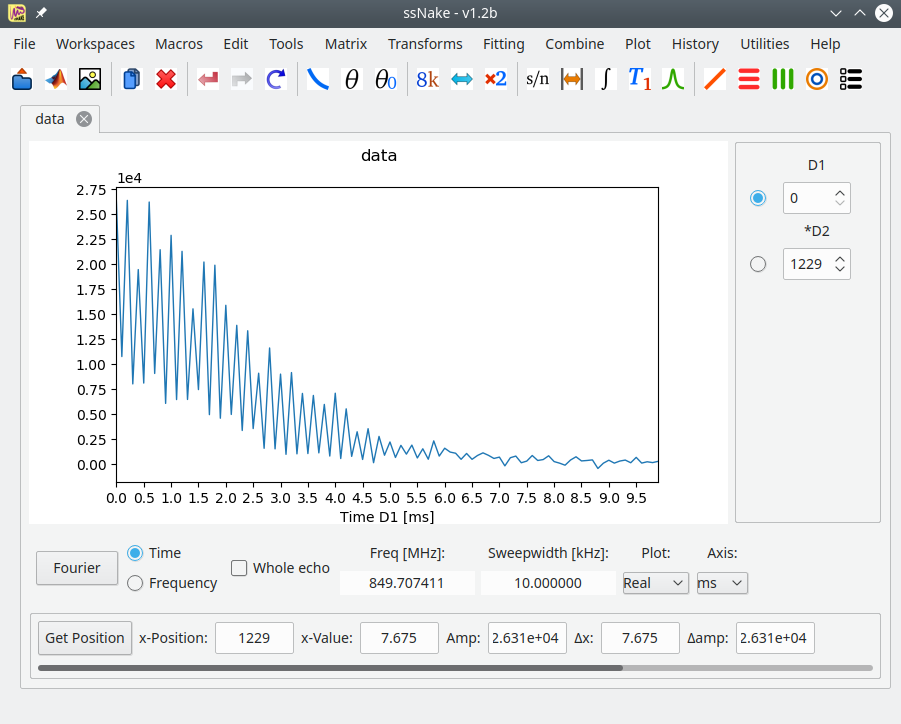
\includegraphics[width=0.8\linewidth]{Figs/Fig1.png}
\end{center}

The rapid oscillations we see here are due to the phase-sensitive recording of
the data (i.e.\ states). We must transforms this data to the hypercomplex
definition:
\begin{itemize}
  \item Convert the States data via `Transforms $\longrightarrow$ Hypercomplex
	 $\longrightarrow$ States'
  \item Take the complex conjugate via `Tools $\longrightarrow$ Complex
	 Conjugate'\footnote{This is required to mirror the spectrum. This is because
	 Varian data uses a different definition for the sign of the imaginary part
  than ssNake.}
\end{itemize}
This should show:
\begin{center}
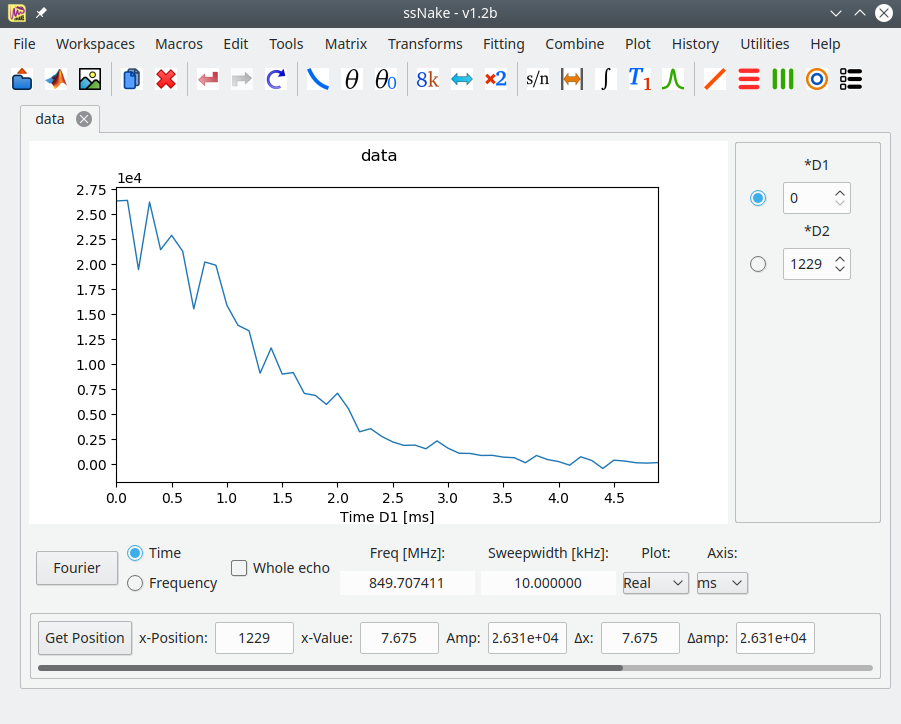
\includegraphics[width=0.8\linewidth]{Figs/Fig2.png}
\end{center}
This looks OK, but actually the time axis is not correct. The current figure
shows the data in the order which they were recorded, not taking the missing
point into account. To correct for this, we must reorder the data, using the
information saved with the experimental data (in `sampling.sch').
\begin{itemize}
  \item Reorder the dating using `Matrix $\longrightarrow$ Reorder', browse for
	 the `sampling.sch' delivered in the data directory of this tutorial, and
	 apply.
\end{itemize}
This should show:
\begin{center}
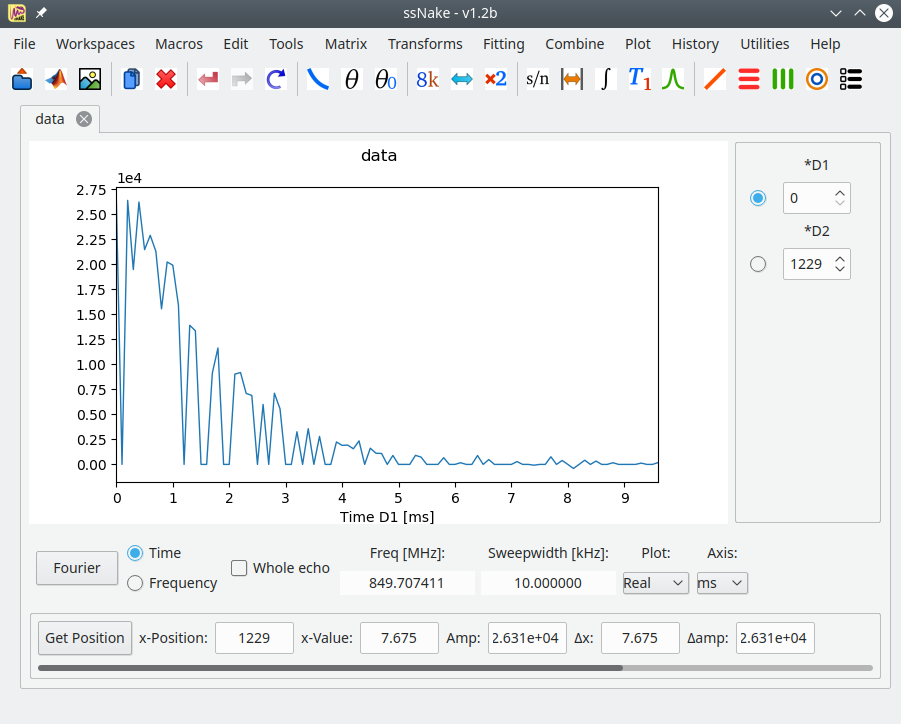
\includegraphics[width=0.8\linewidth]{Figs/Fig3.png}
\end{center}
Here, it can be clearly seen that we have many points which are not recorded:
they are zero. This is essentially what non-uniform sampling entails.

Now that we have our non-uniform `FID', we can start to reconstruct a spectrum
based on this. First, we must phase the data. This is because most
reconstruction algorithms can only accurately reconstruct in-phase data. We will
phase in the spectrum, which will look really bad due to all the zero's in our
FID (we have not yet reconstructed the data).
\begin{itemize}
  \item Fourier transform
  \item Phase with 18.180 degree zero order phasing
  \item Push the Fourier button again (do an inverse transform)
  \item Zerofill to 256 data points using `Matrix $\longrightarrow$ Sizing'
\end{itemize}
Now, we are ready to do a reconstruction. We will use IST (iterative soft
thresholding) in this case. It requires as inputs the threshold ($0 < x <1$, with
closer to 1 slower, but more accurate), the maximum number of steps, and the
stopping condition (percentage of the maximum). The stopping condition should
be roughly the intensity of the noise (no useful information is add after
this point).
\begin{itemize}
  \item Do IST via `Transforms $\longrightarrow$ NUS $\longrightarrow$ IST', put
	 the Threshold at 0.95, and the Max.\ Iterations at 200. Also required is the
	 sampling scheme again:browse for the `sampling.sch'.
\end{itemize}
This shows:
\begin{center}
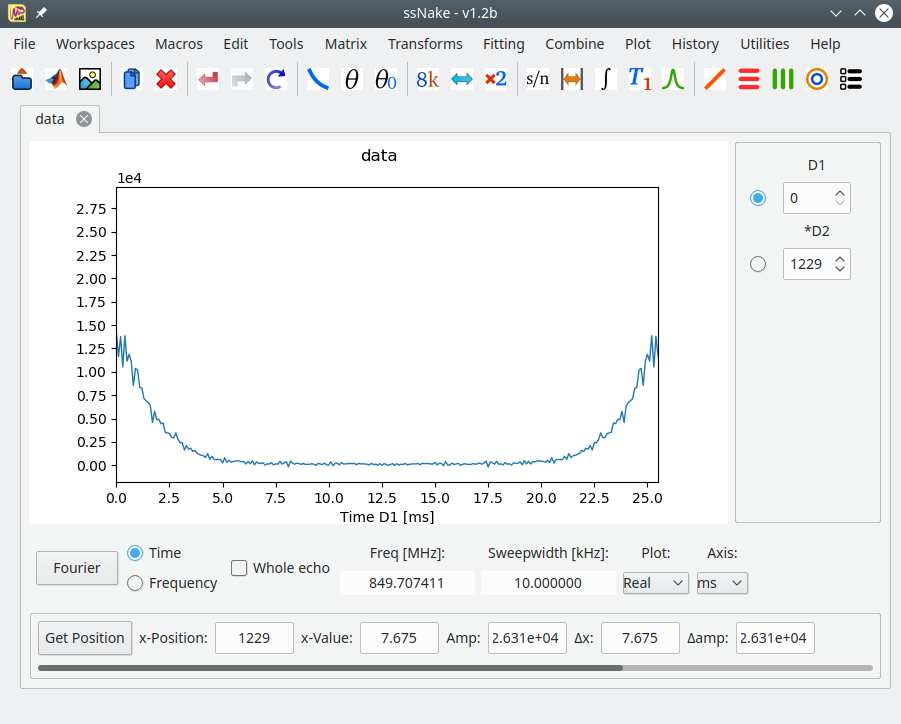
\includegraphics[width=0.8\linewidth]{Figs/Fig4.png}
\end{center}
Which is our reconstructed FID. It looks a bit funny (why is the intensity going
up at the end?). This is due to the fact the we have not reconstructed the
imaginary part of the spectrum in this analysis. We can fix this later on. First
we go to the spectrum:
\begin{itemize}
  \item Push Fourier button
\end{itemize}
This shows:
\begin{center}
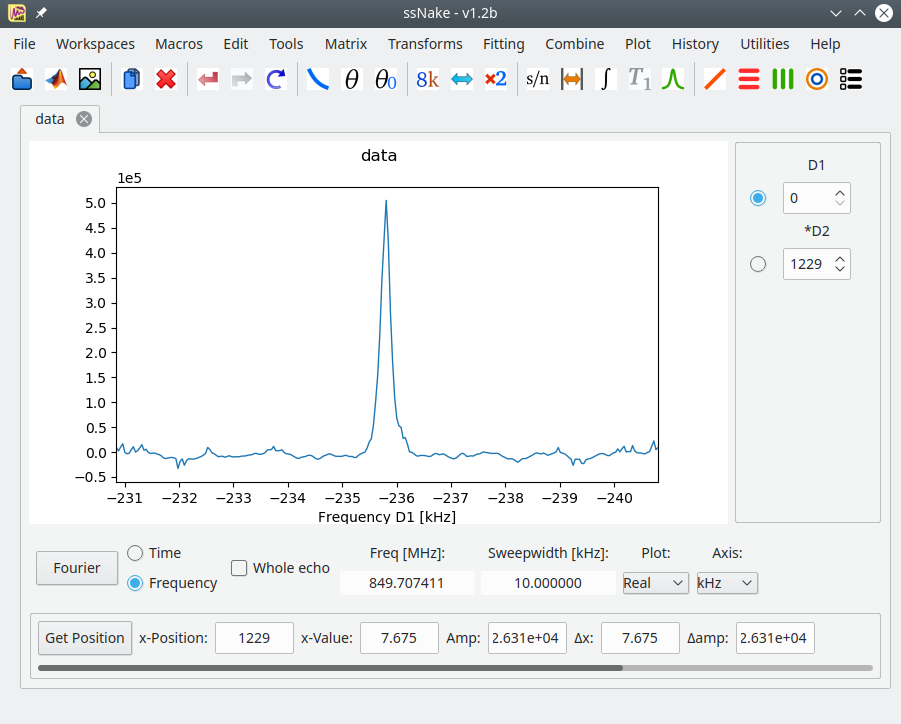
\includegraphics[width=0.8\linewidth]{Figs/Fig5.png}
\end{center}
which is our reconstructed spectrum. This is clearly much better than what we get
without doing the IST:
\begin{center}
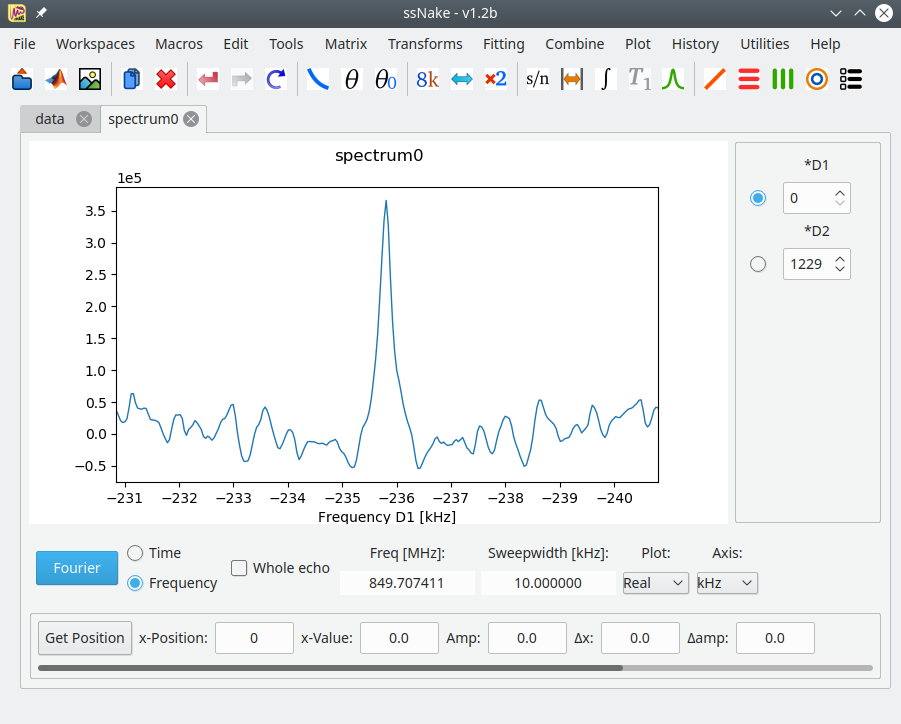
\includegraphics[width=0.8\linewidth]{Figs/Fig6.png}
\end{center}
Plotting the imaginary data also, we see that it is zero:
\begin{center}
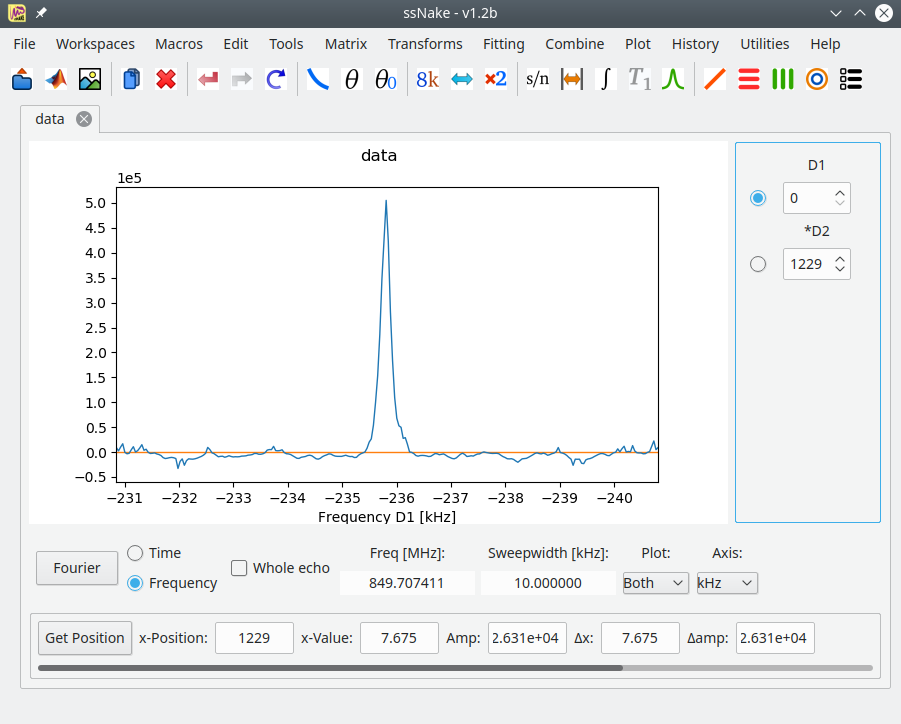
\includegraphics[width=0.8\linewidth]{Figs/Fig7.png}
\end{center}
We decided to not reconstruct the imaginary data by default in ssNake. This is
because imaginary data would allow for phasing, which is not allowed after IST:
only in-phase data can be properly reconstructed. If desired, the imaginary data
can be generated manually, by performing a Hilbert transform:
\begin{itemize}
  \item Do a Hilbert transform via `Transforms $\longrightarrow$ Hilbert
	 Transform'
  \item Take the complex conjugate via `Tools $\longrightarrow$ Complex
	 Conjugate'
\end{itemize}
This shows:
\begin{center}
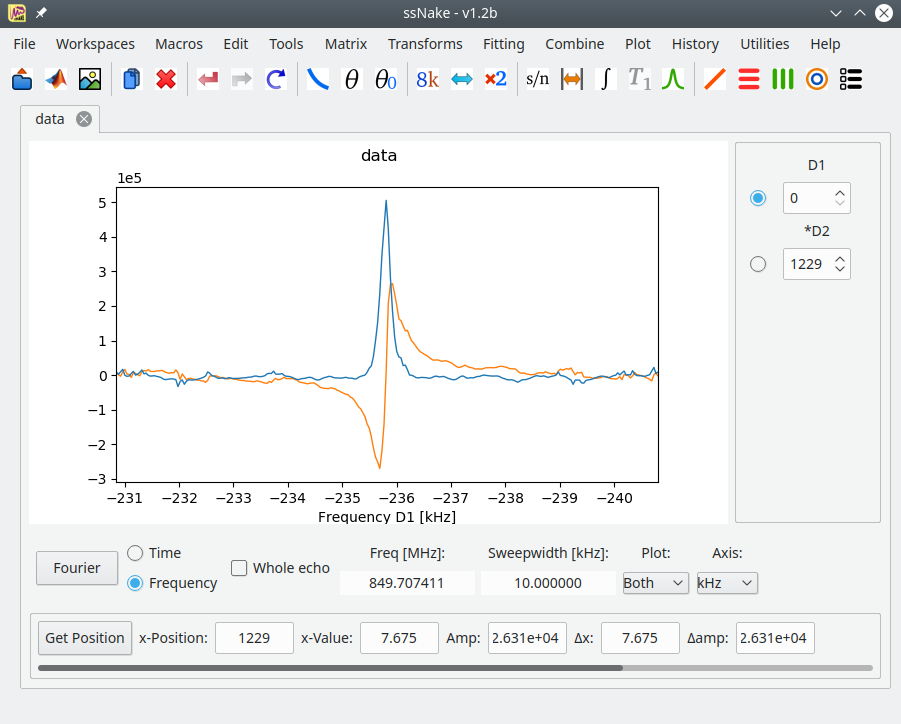
\includegraphics[width=0.8\linewidth]{Figs/Fig8.png}
\end{center}
Doing an inverse Fourier Transform shows an FID as we are used to:
\begin{center}
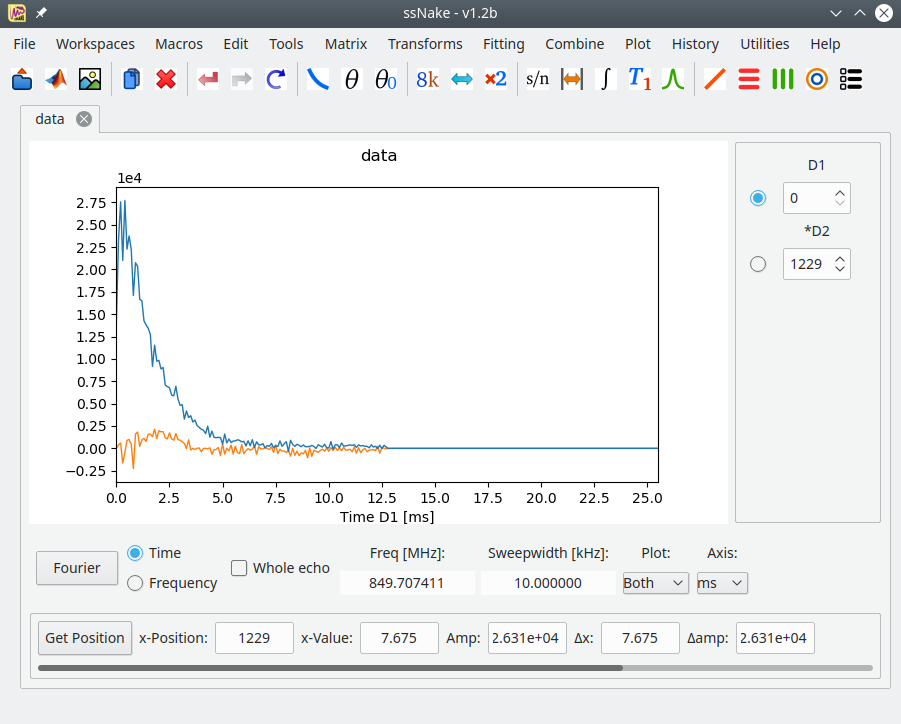
\includegraphics[width=0.8\linewidth]{Figs/Fig9.png}
\end{center}
Finally, we can also view our reconstructed spectrum as a 2D contour plot:
\begin{center}
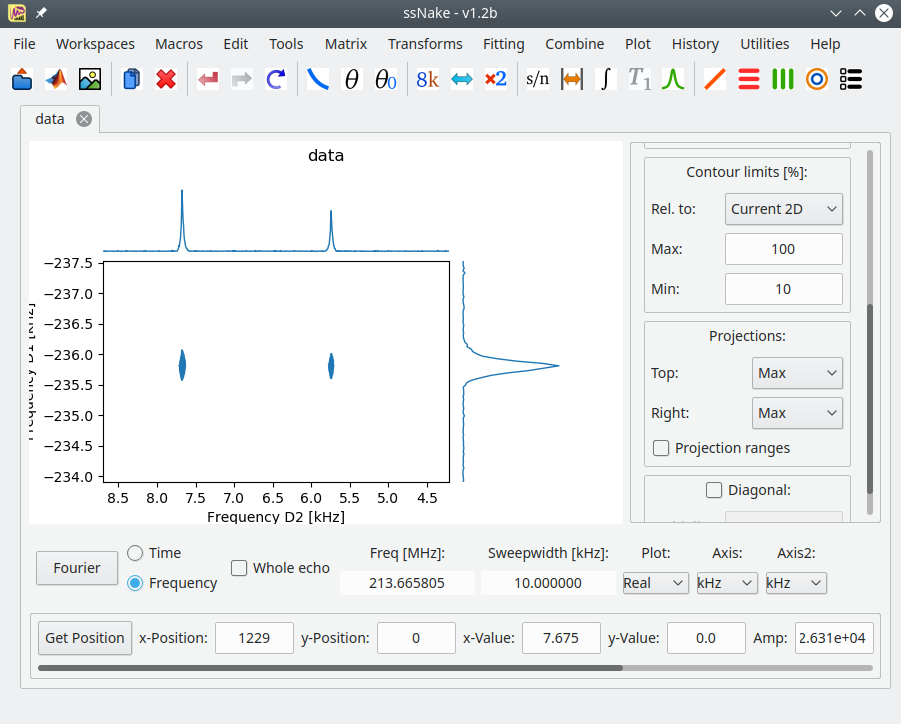
\includegraphics[width=0.8\linewidth]{Figs/Fig10.png}
\end{center}
This concludes this tutorial on NUS processing.


\end{document}
